%-*- coding: utf-8; -*-
\documentclass[a4paper,10pt]{article}
\usepackage[a4paper, top=3cm]{geometry}
\usepackage[utf8]{inputenc}
\usepackage[german]{babel}
\usepackage{fancyhdr}
\usepackage{graphicx}
\usepackage{caption}
\usepackage{amsmath}
\usepackage{amssymb}
\usepackage{pdfpages}
\usepackage{sectsty}
\usepackage{hyperref}

\sectionfont{\fontsize{12}{13}\selectfont}
\captionsetup{font=scriptsize,labelfont=scriptsize}
\pagestyle{fancy}
\setlength{\parindent}{0pt}

\lhead{\small Amateurfunkgruppe der TU Berlin (AfuTUB) \\
       \normalsize \textbf{Ausbildungs-Logbook}}
\chead{}
\rhead{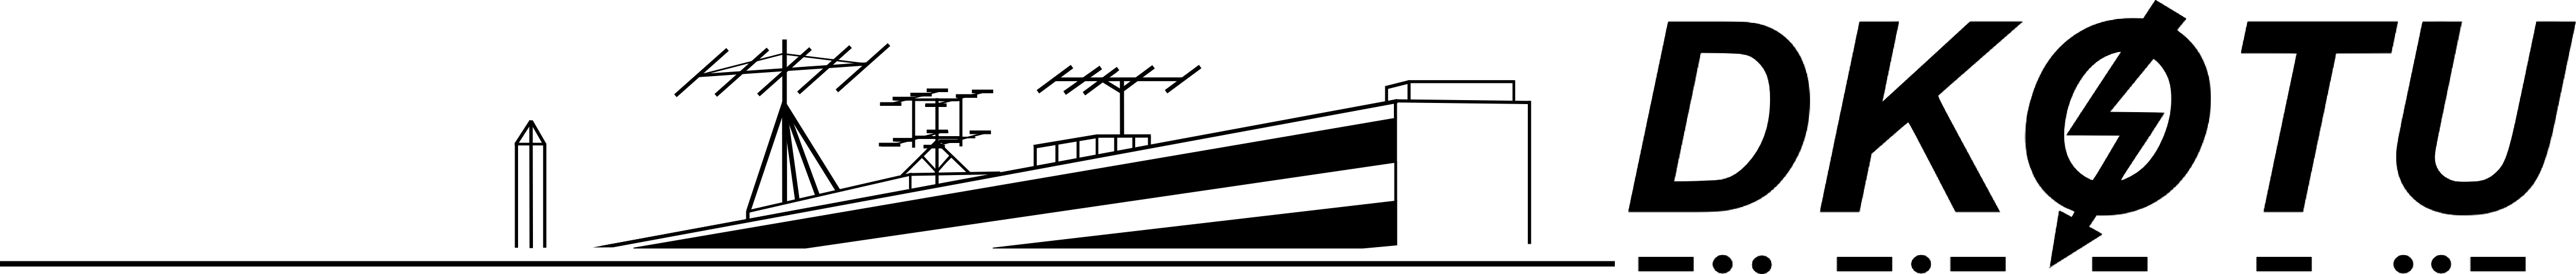
\includegraphics[height=0.9cm]{img/dk0tu-logo_2016-1_rooftop+call_bw.png}}
\lfoot{\footnotesize \it CC BY-NC-SA Sebastian Lange (DL7BST@bastla.net),
       Stand 2016-10-20}
\cfoot{}
\rfoot{\thepage}

\renewcommand{\headrulewidth}{0.0pt}
\renewcommand{\footrulewidth}{0.4pt}

%%%%%%%%%%%%%%%%%%%%%%%%%%%%%%%%%%%%%%%%%%%%%%%%%%%%%%%%%%%%%%%%%%%%%%%%
%% Document

\begin{document}

\begin{center}
    \Large ``Mein erstes QSO''
\end{center}

\vspace{-1.5em}

\section{Abstract}

Um gleich von Beginn an in die Praxis reinzuschnuppern geht es bei den ersten
Funkkontakten (QSO) darum im Nahbereich auf UKW und gut verständlicher
FM-Modulation erste Funksprüche abzusetzen. Im Fokus sind hierbei der Ablauf
eines Funkspruchs, Funkdisziplin sowie das Üben des internationalen
Buchstabieralphabets. Dies dient auch als erste Vorbereitung für die Funkpraxis
auf Kurzwelle in der Clubstation.

\section{Aufgabe}

\textbf{Vorbereitung:} Sucht euch in der Gruppe einen Standort (QTH) und ein
Lösungswort mit der Länge der Anzahl der Teilnehmenden aus. Jede/r bekommt einen
Buchstaben und hat die Aufgabe diesen den anderen Stationen zu übermitteln.
\bigskip

\textbf{Ablauf:} In jeden Durchgang sind das Rufzeichen (Call), das QTH (z.B.
Raumnummer) und der eigene Vorname zu Buchstabieren sowie der Lösungsbuchstabe
und die Stelle im Wort zu übertragen. Jedes QSO ist zu loggen. Eine beliebige
Station startet mit einem allgemeinen Anruf. Nach jedem Durchgang ist die QRG
freizugeben und die zuvor nicht rufende Station darf allgemein oder direkt
anrufen. Alles weitere ergibt sich.

\textit{Hinweis für die Ausbilder: Es ist kein Contest, also bitte piano.}
\bigskip

\textbf{Ziel:} Der Funkplan ist -- inlusive der Lösungswörter -- vollständig
auszufüllen. Tip: Zieht euch Unterstriche für die Anzahl der Personen der
Gegenstelle und füllt es nicht vollständig aus, auch wenn ihr es bereits erraten
könnt.

\section{ITU Phonetic Alphabet \& Notizen}

\hspace{4cm}
\begin{minipage}[t]{0.5\textwidth}
    Calls, Namen, Rapporte, QTH, Zusatzinfos:
    \begin{itemize}
        \item \dots
    \end{itemize}
\end{minipage}

\vspace{-1cm}

\textbf{A}lpha\\
\textbf{B}ravo\\
\textbf{C}harly\\
\textbf{D}elta\\
\textbf{E}cho\\
\textbf{F}oxtrott\\
\textbf{G}olf\\
\textbf{H}otel\\
\textbf{I}ndia\\
\textbf{J}uliett\\
\textbf{K}ilo\\
\textbf{L}ima\\
\textbf{M}ike\\
\textbf{N}ovember\\
\textbf{O}scar\\
\textbf{P}apa\\
\textbf{Q}uebec\\
\textbf{R}omeo\\
\textbf{S}ierra\\
\textbf{T}ango\\
\textbf{U}niform\\
\textbf{V}ictor\\
\textbf{W}hiskey\\
\textbf{X}-Ray\\
\textbf{Y}ankee\\
\textbf{Z}ulu\\

\clearpage

\section{Funkplan}

    \bigskip
    \hspace{8cm}
    \begin{minipage}[t]{0.33\textwidth}
        \centering
        \hrule
        \vspace{0.5ex}
        \small QRG \& Mode
    \end{minipage}

    \begin{center}
    %\footnotesize
    \renewcommand{\arraystretch}{1.5}
    \begin{tabular}{|l|c|l|c|c|c|l|l|}\hline
        \textbf{Call} & \textbf{QTH} & \textbf{\#Pers.} & \textbf{Namen} \\ \hline \hline
        \hspace{1cm} & \hspace{1cm} & & \hspace{10cm} \\ \hline
         & & &  \\ \hline
         & & &  \\ \hline
         & & &  \\ \hline
         & & &  \\ \hline
         & & &  \\ \hline
         & & &  \\ \hline
         & & &  \\ \hline
         & & &  \\ \hline
         & & &  \\ \hline
         & & &  \\ \hline
         & & &  \\ \hline
         & & &  \\ \hline
         & & &  \\ \hline
         & & &  \\ \hline
         & & &  \\ \hline
         & & &  \\ \hline
         & & &  \\ \hline
         & & &  \\ \hline
    \end{tabular}
    \end{center}

\section{Lösungswörter}

\begin{itemize}
    \item Gruppe \hspace{1cm} \dots \hspace{1cm}:
    \item Gruppe \hspace{1cm} \dots \hspace{1cm}:
    \item Gruppe \hspace{1cm} \dots \hspace{1cm}:
    \item Gruppe \hspace{1cm} \dots \hspace{1cm}:
    \item Gruppe \hspace{1cm} \dots \hspace{1cm}:
    \item Gruppe \hspace{1cm} \dots \hspace{1cm}:
    \item Gruppe \hspace{1cm} \dots \hspace{1cm}:
    \item Gruppe \hspace{1cm} \dots \hspace{1cm}:
    \item Gruppe \hspace{1cm} \dots \hspace{1cm}:
    \item Gruppe \hspace{1cm} \dots \hspace{1cm}:
\end{itemize}

\clearpage

\section{Logbook (vereinfacht)}
    \label{att:log0}

    \bigskip
    \hspace{8cm}
    \begin{minipage}[t]{0.33\textwidth}
        \centering
        \hrule
        \vspace{0.5ex}
        \small My Call
    \end{minipage}

    \begin{center}
    %\footnotesize
    \renewcommand{\arraystretch}{1.5}
    \begin{tabular}{|c|c|l|c|l|}\hline
        \textbf{UTC} & \textbf{Band} & \textbf{Call} & \textbf{Mode} & \textbf{SWL} \\ \hline \hline
         ~~1730~~ & 430 & DKØTU & FM & AfuTUBy \\ \hline
         & & \hspace{2cm} & & \hspace{3.0cm} \\ \hline
         & & & & \\ \hline
         & & & & \\ \hline
         & & & & \\ \hline
         & & & & \\ \hline
         & & & & \\ \hline
         & & & & \\ \hline
         & & & & \\ \hline
         & & & & \\ \hline
         & & & & \\ \hline
         & & & & \\ \hline
         & & & & \\ \hline
         & & & & \\ \hline
         & & & & \\ \hline
         & & & & \\ \hline
         & & & & \\ \hline
         & & & & \\ \hline
         & & & & \\ \hline
         & & & & \\ \hline
         & & & & \\ \hline
         & & & & \\ \hline
         & & & & \\ \hline
         & & & & \\ \hline
         & & & & \\ \hline
         & & & & \\ \hline
         & & & & \\ \hline
         & & & & \\ \hline
         & & & & \\ \hline
         & & & & \\ \hline
         & & & & \\ \hline
    \end{tabular}
    \end{center}

    \clearpage

    \begin{center}
    %\footnotesize
    \renewcommand{\arraystretch}{1.5}
    \begin{tabular}{|c|c|l|c|l|}\hline
        \textbf{UTC} & \textbf{Band} & \textbf{Call} & \textbf{Mode} & \textbf{SWL} \\ \hline \hline
         & & \hspace{2cm} & & \hspace{3.0cm} \\ \hline
         & & & & \\ \hline
         & & & & \\ \hline
         & & & & \\ \hline
         & & & & \\ \hline
         & & & & \\ \hline
         & & & & \\ \hline
         & & & & \\ \hline
         & & & & \\ \hline
         & & & & \\ \hline
         & & & & \\ \hline
         & & & & \\ \hline
         & & & & \\ \hline
         & & & & \\ \hline
         & & & & \\ \hline
         & & & & \\ \hline
         & & & & \\ \hline
         & & & & \\ \hline
         & & & & \\ \hline
         & & & & \\ \hline
         & & & & \\ \hline
         & & & & \\ \hline
         & & & & \\ \hline
         & & & & \\ \hline
         & & & & \\ \hline
         & & & & \\ \hline
         & & & & \\ \hline
         & & & & \\ \hline
         & & & & \\ \hline
         & & & & \\ \hline
         & & & & \\ \hline
         & & & & \\ \hline
    \end{tabular}
    \end{center}

    \vspace{8ex}
    \hfill
    %\hspace{0.025\textwidth}
    \begin{minipage}[t]{0.35\textwidth}
        \hrule
        \vspace{0.5ex}
        {\small{Datum,}}\hfill{\small{Unterschrift Rufzeicheninh.}}
    \end{minipage}



\end{document}
